\batchmode
\documentclass{article}
\RequirePackage{ifthen}


\usepackage[english, french]{babel}
\usepackage[utf8]{inputenc}


\title{Lyon Ray Tracer}




\usepackage[dvips]{color}


\pagecolor[gray]{.7}

\usepackage[latin1]{inputenc}



\makeatletter

\makeatletter
\count@=\the\catcode`\_ \catcode`\_=8 
\newenvironment{tex2html_wrap}{}{}%
\catcode`\<=12\catcode`\_=\count@
\newcommand{\providedcommand}[1]{\expandafter\providecommand\csname #1\endcsname}%
\newcommand{\renewedcommand}[1]{\expandafter\providecommand\csname #1\endcsname{}%
  \expandafter\renewcommand\csname #1\endcsname}%
\newcommand{\newedenvironment}[1]{\newenvironment{#1}{}{}\renewenvironment{#1}}%
\let\newedcommand\renewedcommand
\let\renewedenvironment\newedenvironment
\makeatother
\let\mathon=$
\let\mathoff=$
\ifx\AtBeginDocument\undefined \newcommand{\AtBeginDocument}[1]{}\fi
\newbox\sizebox
\setlength{\hoffset}{0pt}\setlength{\voffset}{0pt}
\addtolength{\textheight}{\footskip}\setlength{\footskip}{0pt}
\addtolength{\textheight}{\topmargin}\setlength{\topmargin}{0pt}
\addtolength{\textheight}{\headheight}\setlength{\headheight}{0pt}
\addtolength{\textheight}{\headsep}\setlength{\headsep}{0pt}
\setlength{\textwidth}{349pt}
\newwrite\lthtmlwrite
\makeatletter
\let\realnormalsize=\normalsize
\global\topskip=2sp
\def\preveqno{}\let\real@float=\@float \let\realend@float=\end@float
\def\@float{\let\@savefreelist\@freelist\real@float}
\def\liih@math{\ifmmode$\else\bad@math\fi}
\def\end@float{\realend@float\global\let\@freelist\@savefreelist}
\let\real@dbflt=\@dbflt \let\end@dblfloat=\end@float
\let\@largefloatcheck=\relax
\let\if@boxedmulticols=\iftrue
\def\@dbflt{\let\@savefreelist\@freelist\real@dbflt}
\def\adjustnormalsize{\def\normalsize{\mathsurround=0pt \realnormalsize
 \parindent=0pt\abovedisplayskip=0pt\belowdisplayskip=0pt}%
 \def\phantompar{\csname par\endcsname}\normalsize}%
\def\lthtmltypeout#1{{\let\protect\string \immediate\write\lthtmlwrite{#1}}}%
\newcommand\lthtmlhboxmathA{\adjustnormalsize\setbox\sizebox=\hbox\bgroup\kern.05em }%
\newcommand\lthtmlhboxmathB{\adjustnormalsize\setbox\sizebox=\hbox to\hsize\bgroup\hfill }%
\newcommand\lthtmlvboxmathA{\adjustnormalsize\setbox\sizebox=\vbox\bgroup %
 \let\ifinner=\iffalse \let\)\liih@math }%
\newcommand\lthtmlboxmathZ{\@next\next\@currlist{}{\def\next{\voidb@x}}%
 \expandafter\box\next\egroup}%
\newcommand\lthtmlmathtype[1]{\gdef\lthtmlmathenv{#1}}%
\newcommand\lthtmllogmath{\dimen0\ht\sizebox \advance\dimen0\dp\sizebox
  \ifdim\dimen0>.95\vsize
   \lthtmltypeout{%
*** image for \lthtmlmathenv\space is too tall at \the\dimen0, reducing to .95 vsize ***}%
   \ht\sizebox.95\vsize \dp\sizebox\z@ \fi
  \lthtmltypeout{l2hSize %
:\lthtmlmathenv:\the\ht\sizebox::\the\dp\sizebox::\the\wd\sizebox.\preveqno}}%
\newcommand\lthtmlfigureA[1]{\let\@savefreelist\@freelist
       \lthtmlmathtype{#1}\lthtmlvboxmathA}%
\newcommand\lthtmlpictureA{\bgroup\catcode`\_=8 \lthtmlpictureB}%
\newcommand\lthtmlpictureB[1]{\lthtmlmathtype{#1}\egroup
       \let\@savefreelist\@freelist \lthtmlhboxmathB}%
\newcommand\lthtmlpictureZ[1]{\hfill\lthtmlfigureZ}%
\newcommand\lthtmlfigureZ{\lthtmlboxmathZ\lthtmllogmath\copy\sizebox
       \global\let\@freelist\@savefreelist}%
\newcommand\lthtmldisplayA{\bgroup\catcode`\_=8 \lthtmldisplayAi}%
\newcommand\lthtmldisplayAi[1]{\lthtmlmathtype{#1}\egroup\lthtmlvboxmathA}%
\newcommand\lthtmldisplayB[1]{\edef\preveqno{(\theequation)}%
  \lthtmldisplayA{#1}\let\@eqnnum\relax}%
\newcommand\lthtmldisplayZ{\lthtmlboxmathZ\lthtmllogmath\lthtmlsetmath}%
\newcommand\lthtmlinlinemathA{\bgroup\catcode`\_=8 \lthtmlinlinemathB}
\newcommand\lthtmlinlinemathB[1]{\lthtmlmathtype{#1}\egroup\lthtmlhboxmathA
  \vrule height1.5ex width0pt }%
\newcommand\lthtmlinlineA{\bgroup\catcode`\_=8 \lthtmlinlineB}%
\newcommand\lthtmlinlineB[1]{\lthtmlmathtype{#1}\egroup\lthtmlhboxmathA}%
\newcommand\lthtmlinlineZ{\egroup\expandafter\ifdim\dp\sizebox>0pt %
  \expandafter\centerinlinemath\fi\lthtmllogmath\lthtmlsetinline}
\newcommand\lthtmlinlinemathZ{\egroup\expandafter\ifdim\dp\sizebox>0pt %
  \expandafter\centerinlinemath\fi\lthtmllogmath\lthtmlsetmath}
\newcommand\lthtmlindisplaymathZ{\egroup %
  \centerinlinemath\lthtmllogmath\lthtmlsetmath}
\def\lthtmlsetinline{\hbox{\vrule width.1em \vtop{\vbox{%
  \kern.1em\copy\sizebox}\ifdim\dp\sizebox>0pt\kern.1em\else\kern.3pt\fi
  \ifdim\hsize>\wd\sizebox \hrule depth1pt\fi}}}
\def\lthtmlsetmath{\hbox{\vrule width.1em\kern-.05em\vtop{\vbox{%
  \kern.1em\kern0.8 pt\hbox{\hglue.17em\copy\sizebox\hglue0.8 pt}}\kern.3pt%
  \ifdim\dp\sizebox>0pt\kern.1em\fi \kern0.8 pt%
  \ifdim\hsize>\wd\sizebox \hrule depth1pt\fi}}}
\def\centerinlinemath{%
  \dimen1=\ifdim\ht\sizebox<\dp\sizebox \dp\sizebox\else\ht\sizebox\fi
  \advance\dimen1by.5pt \vrule width0pt height\dimen1 depth\dimen1 
 \dp\sizebox=\dimen1\ht\sizebox=\dimen1\relax}

\def\lthtmlcheckvsize{\ifdim\ht\sizebox<\vsize 
  \ifdim\wd\sizebox<\hsize\expandafter\hfill\fi \expandafter\vfill
  \else\expandafter\vss\fi}%
\providecommand{\selectlanguage}[1]{}%
\makeatletter \tracingstats = 1 


\begin{document}
\pagestyle{empty}\thispagestyle{empty}\lthtmltypeout{}%
\lthtmltypeout{latex2htmlLength hsize=\the\hsize}\lthtmltypeout{}%
\lthtmltypeout{latex2htmlLength vsize=\the\vsize}\lthtmltypeout{}%
\lthtmltypeout{latex2htmlLength hoffset=\the\hoffset}\lthtmltypeout{}%
\lthtmltypeout{latex2htmlLength voffset=\the\voffset}\lthtmltypeout{}%
\lthtmltypeout{latex2htmlLength topmargin=\the\topmargin}\lthtmltypeout{}%
\lthtmltypeout{latex2htmlLength topskip=\the\topskip}\lthtmltypeout{}%
\lthtmltypeout{latex2htmlLength headheight=\the\headheight}\lthtmltypeout{}%
\lthtmltypeout{latex2htmlLength headsep=\the\headsep}\lthtmltypeout{}%
\lthtmltypeout{latex2htmlLength parskip=\the\parskip}\lthtmltypeout{}%
\lthtmltypeout{latex2htmlLength oddsidemargin=\the\oddsidemargin}\lthtmltypeout{}%
\makeatletter
\if@twoside\lthtmltypeout{latex2htmlLength evensidemargin=\the\evensidemargin}%
\else\lthtmltypeout{latex2htmlLength evensidemargin=\the\oddsidemargin}\fi%
\lthtmltypeout{}%
\makeatother
\setcounter{page}{1}
\onecolumn

% !!! IMAGES START HERE !!!

{\newpage\clearpage
\lthtmlfigureA{center21}%
\begin{center}\vbox{\section{Auteur}
Je suis Maxime \textsc{Gaudin}, suis élève ingénieur de l'INSA de Lyon en
échange avec l'École Polytechnique de Montréal (attachée à l'Université de
Montréal).

J'étudie en génie informatique et logiciel.

}\end{center}%
\lthtmlfigureZ
\lthtmlcheckvsize\clearpage}

{\newpage\clearpage
\lthtmlfigureA{center22}%
\begin{center}\vbox{\section{Description}
\subsection{Qu'est ce que c'est ?}
\textsl{Lyon Ray Tracer}, en hommage à ma ville natale : Lyon, est un moteur
de rendu utilisant la technique du \textsl{ray tracing} pour produire des
images photoréalistes. Pour ceux qui ne connaissent pas encore le \textsl{ray
tracing}, je vous invite à consulter notre ami \textsl{Wikipedia}
(\url{http://fr.wikipedia.org/wiki/Lancer_de_rayon}).

Par conséquent, mon moteur prend en entrée des informations comme ``il existe
une sphère de centre (0,0,0) et de rayon 10 qui possède un coefficient de
réflexion de 0.5'', et produit le genre d'image de la figure
\ref{fig:spheres}.

\begin{figure}
\begin{center}
  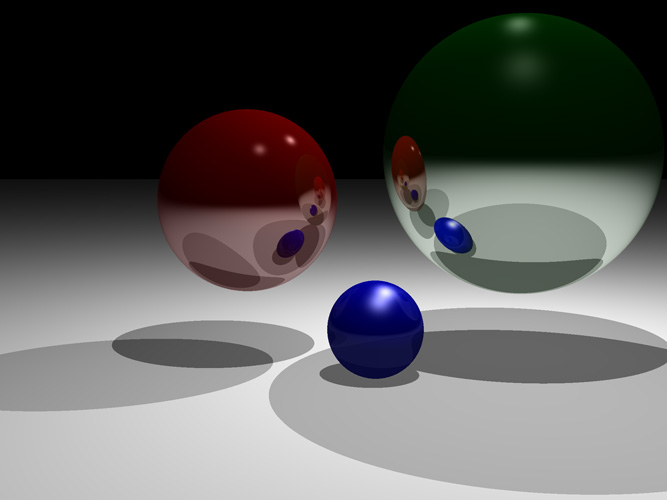
\includegraphics[width=.8\textwidth]{img/spheres}
  \caption{Un exemple de rendu en \textsl{ray tracing}\label{fig:spheres}}
\end{center}
\end{figure}

\subsection{Pourquoi ?}
Bien évidemment parce que j'aime ça ! Mon école ma proposé de réaliser le
projet de mon choix et c'est ce que j'ai choisi. De plus, je trouve que le
concept est formidable : Créer à partir de quelques informations textuelles
des images ultra réalistes et respectant les principes physiques de propagation
de la lumière.

\subsection{Comment ?}
En C++ et en utilisant le plus d'outils libres et standards. Pour vous donner
une idée de mon toolkit, je vous conseil d'aller jeter un coup d'œil du côté
des dépendances.

\subsection{C'est cool, je peux participer ??}
Oh oui !\\

Un moteur de \textsl{ray tracing} c'est comme des Légo, on peu toujours
ajouter quelques choses (surtout en ce moment, puisque le moteur n'est pas
encore très évolué). C'est donc pour toi l'occasion de participer à quelques
choses au tout début de son évolution.\\

Tu peux par exemple :
\begin{itemize}
  \item Me laisser un petit mail pour m'encourager !
  \item Essayer de compiler le programme et m'avertir des différents problèmes
    que tu as pu rencontrer (si possible avec la solution ;) )
  \item M'envoyer des \textsl{pull requests} (même si c'est pour un coquille
    ou ajouter un peu de documentation).
  \item M'aider à créer une vraie page web au lieux de ce PDF :p
\end{itemize}

\subsection{Fonctionnalités}
\paragraph{Lumières}
\begin{itemize}
  \item Lumière directionnelle.
\end{itemize}

\paragraph{Caméra}
\begin{itemize}
  \item Caméra classique avec prise en compte de la perspective.
\end{itemize}

\paragraph{Géométrie}
\begin{itemize}
  \item Sphère.
  \item Plan infini.
\end{itemize}

\paragraph{Matériaux}
\begin{itemize}
  \item Couleur diffuse, spéculaire, ambiante.
  \item Indice de réfraction.
  \item Indice de réflexion.
\end{itemize}

\paragraph{Importeurs}
\begin{itemize}
  \item 3DS.
\end{itemize}

\paragraph{Exporteurs}
\begin{itemize}
  \item PNG.
  \item JPG.
\end{itemize}

}\end{center}%
\lthtmlfigureZ
\lthtmlcheckvsize\clearpage}

{\newpage\clearpage
\lthtmlfigureA{center23}%
\begin{center}\vbox{\section{Dépendences}
La compilation du projet nécessite :
\begin{enumerate}
  \item Un compilateur C++ récent (\textsl{i.e.} gcc 4.2+)
  \item make
  \item boost
  \item libjpeg
  \item libpng
\end{enumerate}

}\end{center}%
\lthtmlfigureZ
\lthtmlcheckvsize\clearpage}

{\newpage\clearpage
\lthtmlfigureA{center24}%
\begin{center}\vbox{\section{Licences}
À priori, LGPL.

}\end{center}%
\lthtmlfigureZ
\lthtmlcheckvsize\clearpage}


\end{document}
